\chapter{Revisão da Literatura}
\label{cap:revisao}

Com o intuito de estabelecer o estado-da-arte acerca dos métodos de percepção veicular baseados em sinais de sensores inerciais, foi conduzida uma Revisão Sistemática da Literatura (RSL) baseada nos procedimentos descritos em \cite{kitchenham2009} e \cite{biolchini2005}. Esta revisão foi publicada em sua forma completa em \cite{menegazzo2018}, com a compilação de dados extraídos dos estudos selecionados e  a descrição detalhada de cada trabalho em ordem cronológica de publicação. Nesta seção, é apresentada a sistemática aplicada na busca e seleção de estudos primários, assim como detalhadas as lacunas de pesquisa encontradas, e que se pretende explorar nesta pesquisa. 

\section{Escopo da Busca}

Na construção do protocolo que guiou a revisão sistemática, foram formuladas as seguintes \textbf{perguntas de pesquisa}:

\begin{enumerate}
\item Quais os métodos aplicados no processamento de sinais de sensores inerciais para gerar percepção veicular?
\item Quais são os padrões reconhecidos e suas classificações?
\item Quais as variáveis utilizadas e os fatores de dependência do modelo?
\item Quais sensores foram utilizados, suas características e configurações? Incluindo sensores não inerciais relacionados aos fatores de dependência.
\item Como os sensores foram distribuídos e posicionados no veículo?
\end{enumerate}

Com estas questões propostas, buscou-se identificar o contexto no qual a amostragem de sinais ocorreu, os sensores utilizados, suas configurações e colocação no veículo. Estas informações são muito importantes para verificar a sensibilidade dos sensores, taxas de amostragem, referenciais e condições gerais de análise. Nos dados amostrados, foram analisadas as etapas de processamento realizadas e quais métodos foram aplicados para pré-processamento de sinais, reorientação de eixos e reconhecimento de padrões. Adicionalmente aos métodos, foram identificados os padrões de percepção veicular, as variáveis dos modelos e seus fatores de dependência, os quais afetam diretamente a adaptabilidade e portabilidade da solução.

\section{Definições da Busca}

Após definir o objeto de pesquisa e o escopo da revisão, foram selecionadas as fontes nas quais os estudos primários foram buscados. A seleção das fontes seguiu os critérios de estar disponível na Internet, ser banco de dados científicos da área e possuir mecanismos avançados de busca baseados na composição lógica de palavras-chave e restrições de campos de documentos. Portanto, três fontes foram selecionadas, detalhadas em Tabela \ref{tabela:definicao_pesquisa}.

Para obter estudos primários a partir das bases de dados científicas definidas, foram construídas inicialmente as \textit{strings} de busca, com base nas palavras-chave obtidas nos estudos de controle. Essas \textit{strings} foram modeladas de acordo com as características de cada fonte. Posteriormente, as \textit{strings} foram submetidas ao respectivo mecanismo de busca e seus resultados analisados por meio de uma estratégia de seleção. No processo de seleção, foram aceitos para a revisão os trabalhos que atenderam a todos os critérios de inclusão e a nenhum dos critérios de exclusão, detalhados na Tabela \ref{tabela:definicao_pesquisa}.

\begin{table}[h!]
    \caption{Definições da busca.}
    \label{tabela:definicao_pesquisa}
    \begin{tabular}{l}
        \toprule
        \textbf{Fontes} \\
        \toprule
        1. IEEE Xplore Digital Library \\
        2. ACM Digital Library \\
        3. Science Direct \\
        \toprule
        \textbf{Critérios de Inclusão}\\
        \toprule
        1. Artigos publicados e disponíveis integralmente em bases de dados científicas digitais.\\
        2. Trabalhos recentes publicados nos últimos sete anos (2013-2019).\\ 
        3. Artigos publicados no idioma inglês.\\
        4. Artigos que reconhecem algum padrão de percepção veicular em sinais de sensores \\ inerciais.\\
        \toprule
        \textbf{Critérios de Exclusão}\\
        \toprule
        1. Artigos que não estão disponíveis integralmente nas fontes pesquisadas.\\
        2. Artigos que não foram publicados nos últimos sete anos (2013-2019).\\
        3. Artigos que não usam sensores inerciais para reconhecimento de padrões.\\
        4. Artigos que não usam sensores inerciais com três eixos.\\
        5. Artigos que não realizam reconhecimento da percepção veicular. \\
        6. Artigos de sensoriamento inercial para veículos de qualquer tração que não sejam \\ mecânicos. \\
        7. Artigos que usam tecnologias intrusivas ou ativas.\\
        8. Artigos em outros idiomas, não incluídos no protocolo.\\
        \bottomrule
    \end{tabular}
    \fonte{O autor.}
\end{table}

\section{Execução da Busca}

Com as definições estabelecidas, foram realizadas buscas por estudos primários nas três fontes selecionadas. Devido à limitação de número de termos nos mecanismos de busca, foram realizadas duas buscas, uma para percepção veicular de ambiente e outra para propriocepção veicular. As \textit{strings} de busca construídas e seus filtros definidos são detalhados nas Tabelas \ref{tabela:percepcao_ambiente_busca} e \ref{tabela:propriocepcao_busca}.

\begin{table}[h!]
    \caption{\textit{Strings} de busca para percepção veicular de ambiente.}
    \label{tabela:percepcao_ambiente_busca}
    \centering
    \begin{tabular}{l l}
        
        \toprule
        \textbf{Fonte} & IEEE Xplore Digital Library \\
        \midrule
        \textbf{String} & ((Road \textbf{OR} Pavement \textbf{OR} Pothole \textbf{OR} Hole \textbf{OR} \\ \textbf{de Busca} & Bump \textbf{OR} "Speed Breaker")  \textbf{AND} (Accelerometer \\ & \textbf{OR} Gyroscope \textbf{OR} "Inertial Sensor")) \\
        \midrule
        \textbf{Filtros} & Range: 2013-2019. Search metadata only. \\
        \bottomrule
        
        \\
        
        \toprule
        \textbf{Fonte} & ACM Digital Library \\
        \midrule
        \textbf{String} & ((Road \textbf{OR} Pavement \textbf{OR} Pothole \textbf{OR} Bump \textbf{OR} \\ \textbf{de Busca} & "Speed Breaker") \textbf{AND} (Accelerometer \textbf{OR} Gyroscope \\ & \textbf{OR} "Inertial Sensor")) \\
        \midrule
        \textbf{Filtros} & Range: 2013-2019. Search in titles and abstracts. \\ 
        \bottomrule
        
        \\
        
        \toprule
        \textbf{Fonte} & Science Direct \\
        \midrule
        \textbf{String} & ((Road \textbf{OR} Pavement \textbf{OR} Pothole \textbf{OR} Hole \textbf{OR} \\ \textbf{de Busca} & Bump \textbf{OR} "Speed Breaker") \textbf{AND} (Accelerometer \\ & \textbf{OR} Gyroscope \textbf{OR} "Inertial Sensor")) \\
        \midrule
        \textbf{Filtros} & Range: 2013-2019. Search in title, abstract and keywords. \\
        \bottomrule
    \end{tabular}
\end{table}

\begin{table}[h!]
    \caption{\textit{Strings} de busca para propriocepção veicular.}
    \label{tabela:propriocepcao_busca}
    \centering
    \begin{tabular}{l l}
        
        \toprule
        \textbf{Source} & IEEE Xplore Digital Library \\
        \toprule
        \textbf{Search} & (Driving Events \textbf{OR} Driving Patterns \textbf{OR} Driving Style \textbf{OR} \\ \textbf{String} & Drive Behaviour) \textbf{AND} (Accelerometer \textbf{OR} Gyroscope \textbf{OR} \\ & “Inertial Sensor”) \\
        \toprule
        \textbf{Filters} & Range: 2013-2019. Search metadata only. \\
        \bottomrule
        
        \\
        
        \toprule
        \textbf{Source} & ACM Digital Library \\
        \toprule
        \textbf{Search} & ("Driving Events" \textbf{OR} "Driving Patterns" \textbf{OR} "Driving Style" \\ \textbf{String} & \textbf{OR} "Drive Behaviour")  \textbf{AND} (Accelerometer \textbf{OR} Gyroscope \\ & \textbf{OR} "Inertial Sensor") \\
        \toprule
        \textbf{Filters} & Range: 2013-2019. Search in titles and abstracts. \\
        \bottomrule
         
         \\
         
        \toprule
        \textbf{Source} & Science Direct \\
        \toprule
        \textbf{Search} & (Driving Events \textbf{OR} Driving Patterns \textbf{OR} Driving Style \textbf{OR} \\ \textbf{String} & Drive Behaviour) \textbf{AND} (Accelerometer \textbf{OR} Gyroscope \textbf{OR} \\ & “Inertial Sensor”) \\
        \toprule
        \textbf{Filters} & Range: 2013-2019. Search in title, abstract and keywords. \\
        \bottomrule
        
    \end{tabular}
\end{table}

\section{Resultados e Discussão}

A busca por percepção de ambiente resultou em 737 artigos e a propriocepção em 239 artigos. Após análise dos estudos de acordo com os critérios estabelecidos, 66 artigos sobre percepção de ambiente e 25 sobre propriocepção foram selecionados para esta revisão, conforme detalhado na Tabela \ref{tabela:resultados_sumarizados_busca}. Com a produção da RSL, diversas lacunas de pesquisa foram encontradas \cite{menegazzo2018}. Nesta seção, são apresentadas e discutidas somente aquelas relacionadas ao escopo deste trabalho. 

\begin{table}[h]
    \caption{Summarized Search Results.}
    \label{tabela:resultados_sumarizados_busca}
    \centering
    \begin{tabular}{l c c c c}
        \toprule
        & \multicolumn{2}{l}{\textbf{Percepção de Ambiente}} & \multicolumn{2}{l}{\textbf{Propriocepção}} \\
        \toprule
        & Recuperado & Selecionado & Recuperado & Selecionado \\
        \toprule
        \textbf{IEEE} & 619 & 51 & 196 & 21 \\
        \midrule
        \textbf{ACM} & 32 & 6 & 6 & 1 \\
        \midrule
        \textbf{Science Direct} & 86 & 9 & 37 & 3 \\
        \toprule
        Total & 737 & 66 & 239 & 25 \\
        \bottomrule
    \end{tabular}
    \fonte{O autor.}
\end{table}

Os estudos selecionados para revisão foram analisados em três etapas, sendo elas a amostragem de dados, pré-processamento e processamento. Na primeira etapa, a coleta de dados nos estudos analisados foi realizada em diferentes contextos, de acordo com o tipo de percepção que se pretendia produzir. Esses contextos envolviam estradas com diferentes pavimentos, estados de conservação, condições climáticas, irregularidades, obstáculos e modos de condução. A utilização de sensores inerciais para gerar percepção veicular se deu na proporção de 70\% utilizando apenas acelerômetro, 27\% utilizando acelerômetro e giroscópio, e 3\% utilizando apenas giroscópio. Neste sentido, a grande utilização de acelerômetro ocorre não por um critério de qualidade, mas em função de ser mais facilmente encontrado em dispositivos móveis que o giroscópio. Contudo, é necessário avaliar qual sensor fornece dados melhores para prover percepção, e se a combinação de ambos pode melhorar os resultados dos modelos propostos.

Os trabalhos foram agrupados de acordo com a plataforma utilizada. Aproximadamente 83\% dos estudos utilizou sensores inerciais embarcados em dispositivos móveis como \textit{smartphones} e \textit{tablets}, enquanto que apenas 17\% utilizaram anexado aos veículos. No uso de sensores em dispositivos móveis, as soluções propostas são mais vulneráveis a erros, pois os dispositivos não permanecem fixos o tempo todo, dependem de uma reorientação dos eixos e, geralmente, possuem sensores menos robustos. Em geral, essa abordagem tem sido utilizada em sistemas de \textit{mobile crowdsensing}, onde os dados produzidos localmente são enviados para um servidor remoto, que recebe percepções veiculares de várias fontes. Após o pós-processamento para melhorar a confiabilidade dos dados, as percepções retornam aos usuários em aplicativos de assistência ao motorista. Por sua vez, o uso de sensores anexados à veículos foi combinado com o utilização de \textit{Single-Board Computer} (SBC), como as placas de prototipagem Raspberry Pi, ou microcontrolador, como o Arduino, visando principalmente resultados locais com maior precisão e acurácia, sem a necessidade de processamento remoto ou dados de outras fontes.

Os sensores foram colocados no veículo de acordo com a plataforma utilizada. Sensores inerciais em dispositivos móveis foram colocados dentro da cabine geralmente na \textit{dashboard}, bancos, próximo ao câmbio de marchas ou fixado com suporte no pára-brisas. Sensores embarcados no veículo foram colocados na \textit{dashboard}, no chassis, dentro da roda, próximo e abaixo da suspensão e próximo e acima da suspensão. A Figura \ref{fig:sensor_placement_ocurrence} detalha os colocações encontradas. Devido à economia de recursos, especialmente a bateria, os dados dos sensores de dispositivos móveis foram coletados a uma taxa de amostragem na faixa de Hz, enquanto aqueles embutidos no veículo utilizaram uma amostragem maior, na faixa de KHz. Os estudos também utilizaram fontes de dados auxiliares, como magnetômetros, GPS e \textit{On-Board Diagnostic} II (OBD-II).

\begin{figure}[h!]
  \centering
  \caption{Colocação dos sensores no veículo.}
   \label{fig:sensor_placement_ocurrence}
   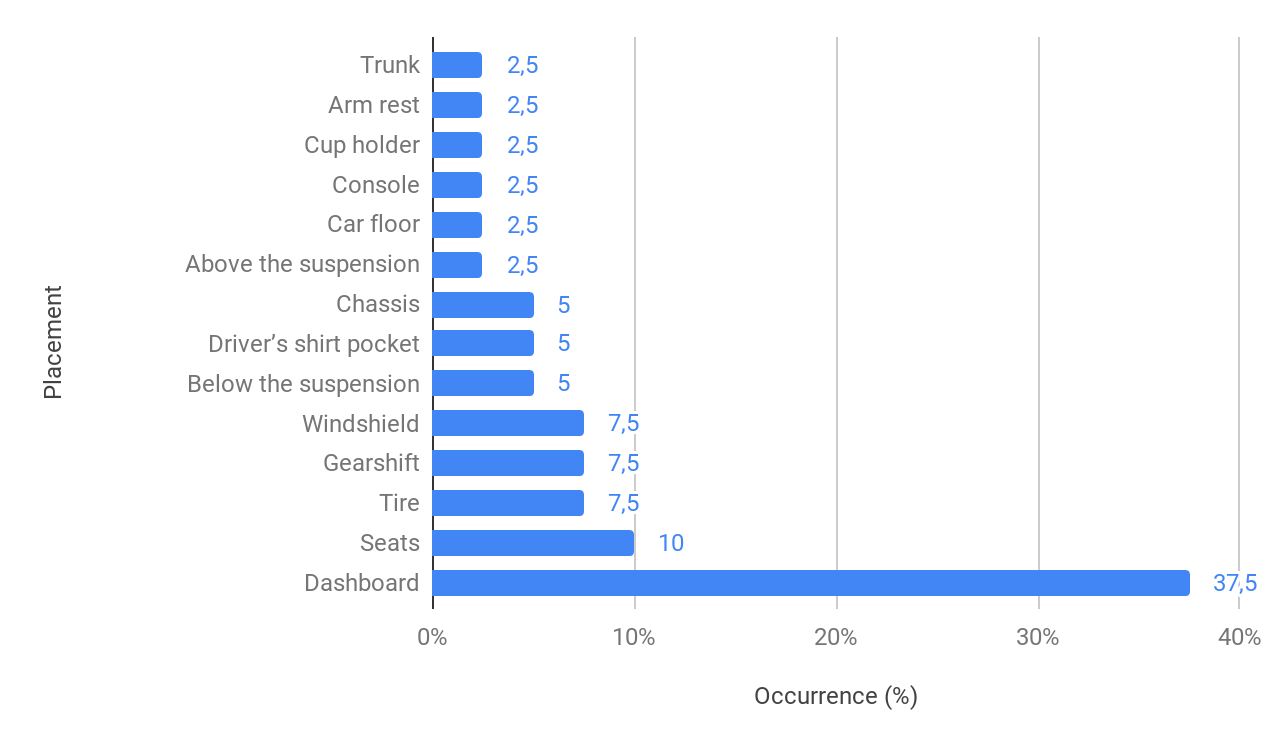
\includegraphics[width=1\textwidth]{figuras/fig3_1.png}
   \fonte{O Autor.}
\end{figure}

Neste contexto, a etapa de coleta de dados apresenta diversas lacunas. Como detalhado anteriormente, se faz necessário analisar a combinação dos dados de ambos os sensores inerciais, e não apenas o mais popular. Em seguida, é necessário buscar taxas de amostragem que não sejam arbitrárias, que permitam a identificação das percepções de forma acurada, utilizando o mínimo necessário de recursos computacionais. Em relação ao colocação dos sensores, como existem fatores de dependência relacionados aos dados do sensor, sua captura em diferentes locais do veículo implica diferentes valores observados para um mesmo evento. Não foram encontrados estudos que correlacionem os sinais em diferentes partes do veículo, a fim de verificar uma possível variação na confiabilidade do reconhecimento devido à colocação do sensor, nem estudos que utilizem dados em mais de uma extremidade do eixo veicular com o intuito de verificar melhoria nos resultados. Por fim, a maior lacuna reside em não haver disponível publicamente bases de dados destes sensores, para se realizar novas pesquisas ou comparar métodos propostos. Além disso, para serem realmente úteis, bases disponíveis para estudos futuros devem seguir toda uma metodologia de colocação de sensores, tanto em relação ao alinhamento como em qual parte do veículo, etapas geralmente pouco exploradas pelos estudos.

Na etapa subsequente, os dados brutos coletados foram pré-processados para serem parametrizados a técnica que reconhece e/ou classifica os padrões de percepção. O pré-processamento foi subdividido em três fases, de acordo com sua finalidade. No primeiro, pré-processamento de sinais, foram aplicados métodos na remoção de ruído, suavização de sinal, segmentação e extração de características. No segundo, foram aplicados métodos para a reorientação de eixos. Finalmente, na terceira fase, foram aplicados métodos para georreferenciamento dos dados.

As técnicas aplicadas no pré-processamento dos sinais, mostradas na Figura \ref{fig:signal_preprocessing} foram utilizadas principalmente no domínio do tempo, embora outros domínios como frequência e tempo-frequência também tenham sido explorados. Abordagens estatísticas como Gaussian \cite{Pooja2017}, Skewness \cite{Alqudah2016}, Kurtosis \cite{Alqudah2016}, Median \cite{Alqudah2016,Li2016}, Root Mean Square (RMS) \cite{Jang2015,Li2018,Sharma2015}, Moving Average/Average \cite{Alqudah2016,Andria2016,Bose2018,Li2016, Pholprasit2015,Savera2016,Singh2017}, Moving Variance/Variance \cite{Alqudah2016,Andria2016} e Standard Deviation \cite{Andria2016,BelloSalau2018,Hou2017,Lima2016,Pholprasit2015,Prapulla2017} foram utilizados no domínio do tempo para suavizar os sinais e extrair características dos dados de vibração. Cerca de 60\% dos estudos analisados utilizaram estes métodos estatísticos.

\begin{figure}[h!]
  \centering
  \caption{Métodos utilizados no pré-processamento de sinais.}
   \label{fig:signal_preprocessing}
   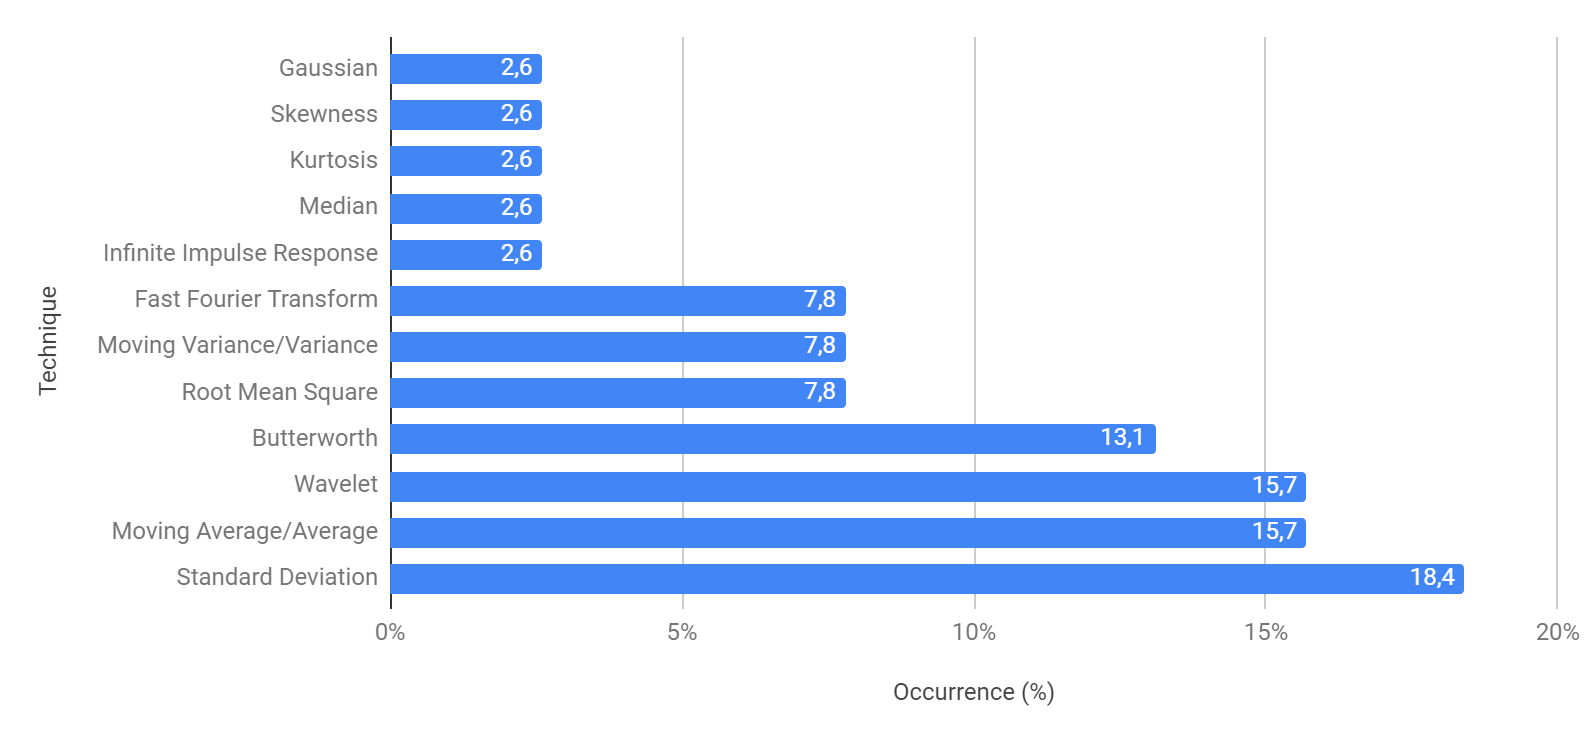
\includegraphics[width=1\textwidth]{figuras/fig3_2.png}
   \fonte{O Autor.}
\end{figure}

No domínio da frequência, os filtros Infinite Impulse Response \cite{Wu2018} e Butterworth \cite{Hou2017,Niskanen2015,Pitonak2016,Souza2018,Wu2013} foram utilizados na remoção de componentes dos sinais. Já a Fast Fourier Transform (FFT) \cite{Allouch2017,Douangphachanh2013,Douangphachanh2014} e Wavelets \cite{BelloSalau2018,Eftekhari2018,El-Wakeel2018,Gueta2017,Singh2017,Wang2018} foram utilizadas na remoção de ruídos e extração de características. A segmentação dos dados foi realizada em quadros deslizantes em função do tempo \cite{Wang2018}, número de amostras \cite{Singh2017} ou distância \cite{Li2018}.

Após o pré-processamento de sinais, alguns estudos utilizaram a reorientação de eixos entre os sistemas de coordenadas, mapeando os dados do referencial do sensor para o referencial do veículo. Entre os que utilizaram, a maioria empregou fórmulas baseadas nos ângulos de Euler \cite{Li2018, Orhan2013, Singh2017, Vittorio2014, Vlahogianni2017}. Os ângulos foram calculados de diferentes maneiras. Em \cite{Singh2017, Orhan2013, Vittorio2014} o referencial inicial foi estabelecido como estado estacionário ($x=0m/s^2$, $y=0m/s^2$ e $z=9.81m/s^2$), a partir dos qual os ângulos de mapeamento foram calculados. Em \cite{Li2018} foi utilizado como estado inicial os valores do acelerômetro, medindo os ângulos continuamente. \cite{Singh2018} usou como estado inicial as médias individuais dos valores de aceleração nos três eixos, dos últimos 15 segundos, quando a magnitude total estava próxima de $9.8 \pm 0.2 m/s^2$. Todos eles empregaram como orientação final os valores atuais de aceleração.

As três formas apresentadas para o cálculo dos ângulos de Euler possuem limitações pontuais. Na primeira, devido a utilização de uma orientação inicial que não é atualizada continuamente, os valores em locais com inclinação do solo podem apresentar erros. Isso se deve ao fato de que nesses locais a força da aceleração gravitacional se distribui entre os eixos, não sendo isolada no eixo de aceleração vertical. Na segunda técnica, embora os ângulos sejam atualizados, o valor da gravidade não é isolada e pode levar a erros uma vez que não é o único componente de força presente nos eixos. Na terceira técnica, devido à tentativa de identificar um possível estado estacionário durante o curso do veículo para defini-lo como um novo estado inicial, implica que os trajetos de alta vibração não satisfaçam as condições e não atualizem os ângulos, acumulando erros. 

Todos os métodos apresentados de cálculo de ângulos de Euler para reorientação de eixos são baseadas na localização da força de aceleração gravitacional. Sendo assim, a partir de um estado estacionário inicial, sua orientação final também deve ser estacionária e não relativa os dados atuais de aceleração. Ainda baseadas na gravidade, as técnicas reorientam o eixo Z perpendicular ao solo, apontando para o céu, ao invés de serem perpendiculares ao veículo. Logo, os dados são reorientados para o referencial do mundo real e não no do veículo, sendo que estes somente sobrepõe o eixo Z em casos de trajeto plano. Este tipo de reorientação é útil apenas quando utilizado em dispositivos móveis e sistemas de \textit{crowdsourcing}, produzindo apenas percepção de ambiente. Para propriocepção, mesmo adicionando orientação com o magnetômetro, o referencial do mundo real não permite identificar os eventos de condução, sendo necessário estar no referencial do veículo. Portanto, a abordagem de posicionamento controlado, embora simples, com a fixação dos sensores e alinhamento de eixos apresenta menor possibilidade de erros, permitindo percepção de ambiente e propriocepção.

Ainda na etapa de pré-processamento, uma vez que a taxa de amostragem de dados dos sensores inerciais é muito mais rápida que a amostragem de dados de localização (1Hz), são necessárias técnicas para estimar a localização e velocidade antes da próxima amostra do GPS. Para isso, apenas \cite{Li2018} utilizou um tratamento, aplicando interpolação linear com os dados de aceleração para obter dados de localização com mais frequência. Contudo, o mesmo não foi feito com a velocidade. O desenvolvimento de um método com este intuito é de extrema importância uma vez que a velocidade constitui um fator de dependência e deve ser a mais próxima da real possível. Da mesma forma, estimar os pontos de localização auxilia a mitigar pontos cegos, dentre outros problemas.

\begin{figure}[h!]
  \centering
  \caption{Técnicas para reconhecimento e/ou classificação de padrões.}
   \label{fig:techniques_occurrence}
   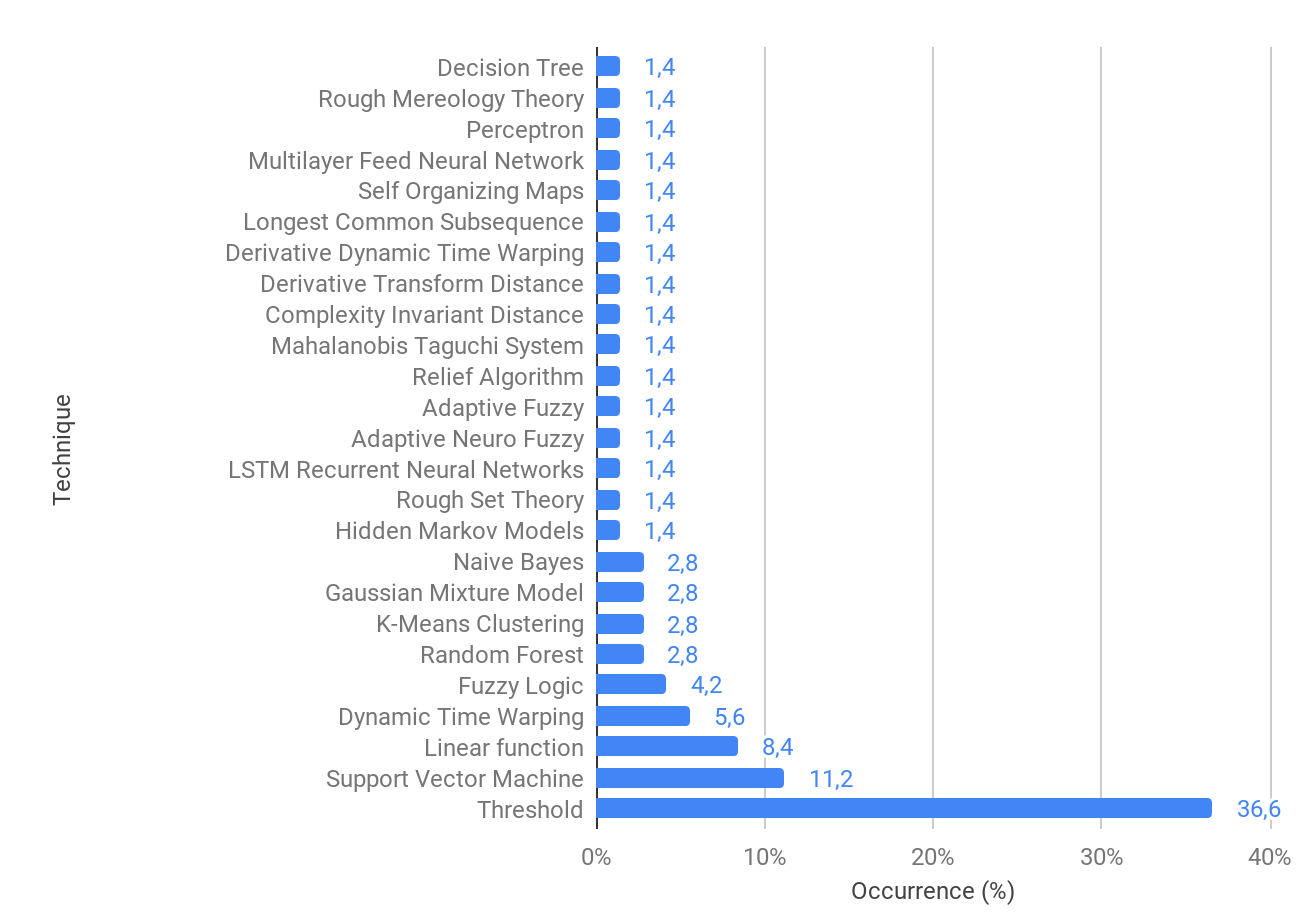
\includegraphics[width=0.95\textwidth]{figuras/fig3_3.png}
   \fonte{O autor.}
\end{figure}

Para reconhecer e classificar os padrões nos dados pré-processados dos sensores inerciais, várias técnicas foram propostas, conforme detalhado na Figura \ref{fig:techniques_occurrence}. Essas técnicas foram classificadas de acordo com sua abordagem.  Embora alguns trabalhos apresentem técnicas com abordagens mais elaboradas, como métodos de alinhamento de séries temporais, aprendizado de máquina e modelos com conhecimento especialista, quase metade deles utiliza técnicas extremamente simples, como limiares e funções lineares. Abordagens mais recentes, como o \textit{Deep Learning}, foram encontradas em apenas um estudo, o qual se limita a um tipo de percepção. Os resultados dos métodos não foram comparados na revisão, devido a poucos apresentarem resultados numéricos, bem como pelo uso de uma diversidade de cenários e técnicas não adaptativas, não permitindo uma comparação direta.

Através da análise dos estudos, observou-se um foco maior na simples e imediata aplicabilidade do que no fornecimento de dados mais precisos e acurados com certo grau de adaptabilidade. Sendo assim, a maioria dos trabalhos se concentra na aplicabilidade direta, e a adaptabilidade das soluções apresentadas é mínima, sendo o principal obstáculo para seu amplo uso em cenários do mundo real. Relacionada aos fatores de dependência, a adaptabilidade raramente é mencionada nos trabalhos. Alguns estudos agregaram em seus modelos o fator de velocidade ou o modelo \textit{Quarter Car} \cite{Tomiyama2016}, contudo nenhum deles trata todos os fatores de dependência, para produzir diversos tipos de percepção. \cite{Singh2017} argumenta que não é possível cobrir todas as condições através do aprendizado de máquina e dos modelos de limiares existentes. No entanto, a adaptabilidade deve ser investigada do ponto de vista das três etapas apresentadas, especialmente integrando os dados às novas e robustas técnicas de aprendizado de máquina. Outro ponto a ser explorado no sentido da adaptabilidade e ainda não observado nos estudos é a integração dos dados de percepção, uma vez que todos são inter relacionados, seja de percepção de ambiente ou propriocepção.

Finalmente, vários tipos de dados de percepção foram identificados pelos estudos analisados nesta revisão. Além da classificação entre a percepção do ambiente e a propriocepção, as percepções também foram classificadas quanto ao momento de detecção, sendo eventos transientes aqueles detectados momentaneamente, e eventos persistentes aqueles que ocorrem a todo o momento. Sendo assim, na percepção do ambiente, são considerados eventos transientes obstáculos na estrada e anomalias de superfície, e eventos persistentes a identificação do tipo de pavimento, os índices de irregularidade e os níveis de qualidade. Na propriocepção, eventos transientes são eventos de condução e eventos persistentes são relacionados ao perfil do comportamento de condução. As figuras \ref{fig:environment_perception_occurrence} e \ref{fig:proprioception_occurrence} detalham as percepções encontradas.

\begin{figure}[h!]
  \centering
  \caption{Percepções de ambiente encontradas nos estudos analisados.}
   \label{fig:environment_perception_occurrence}
   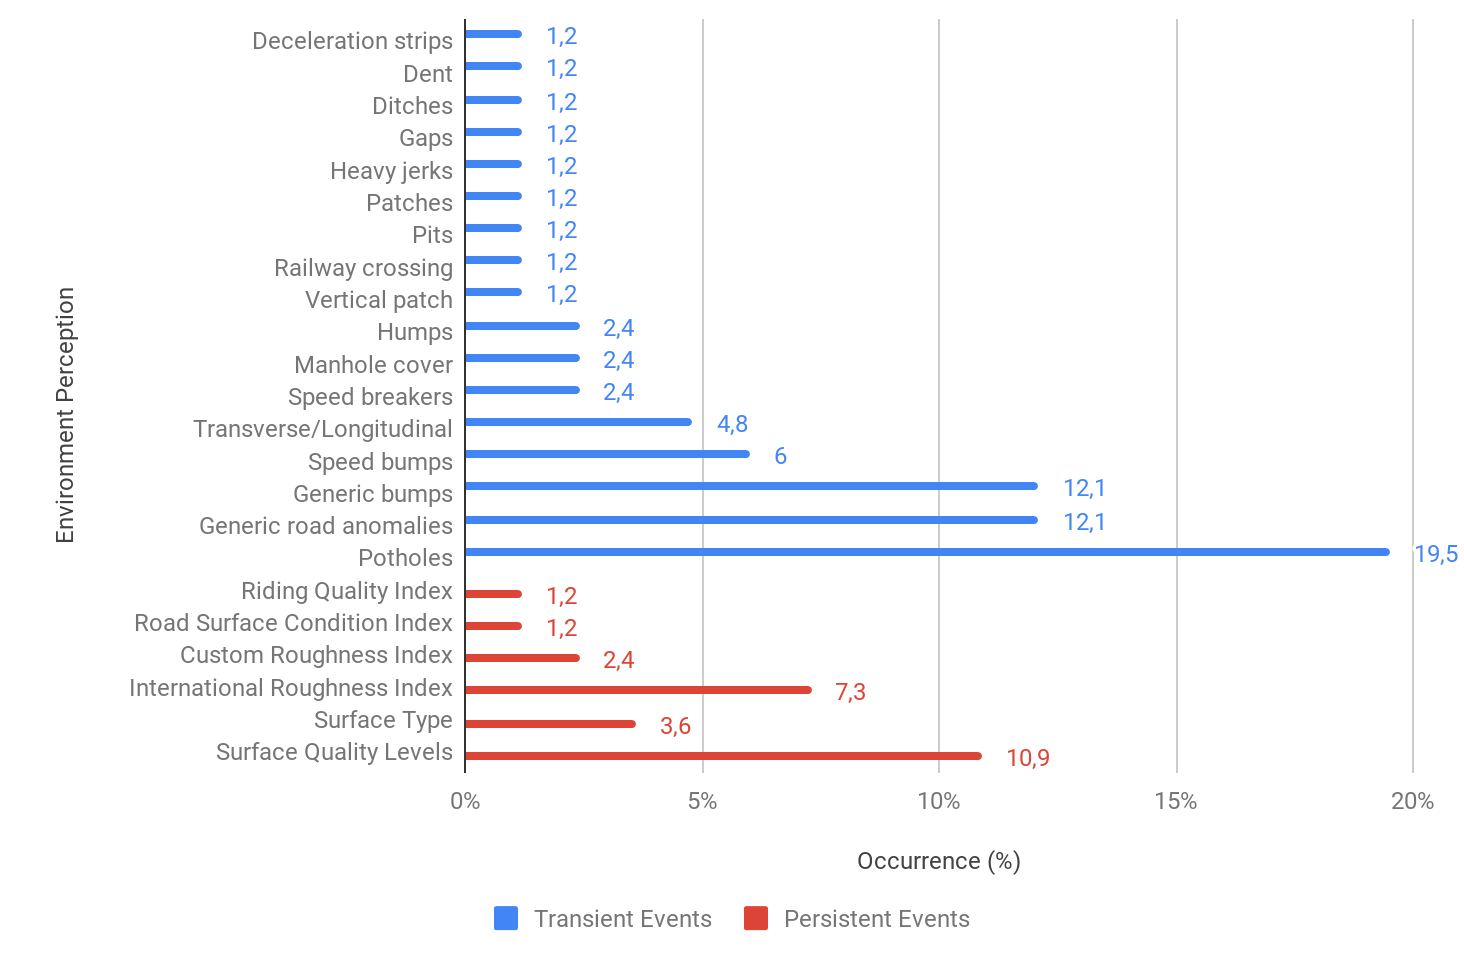
\includegraphics[width=0.95\textwidth]{figuras/fig3_4.png}
   \fonte{O autor.}
\end{figure}

\begin{figure}[h!]
  \centering
  \caption{Propriocepções encontradas nos estudos analisados.}
   \label{fig:proprioception_occurrence}
   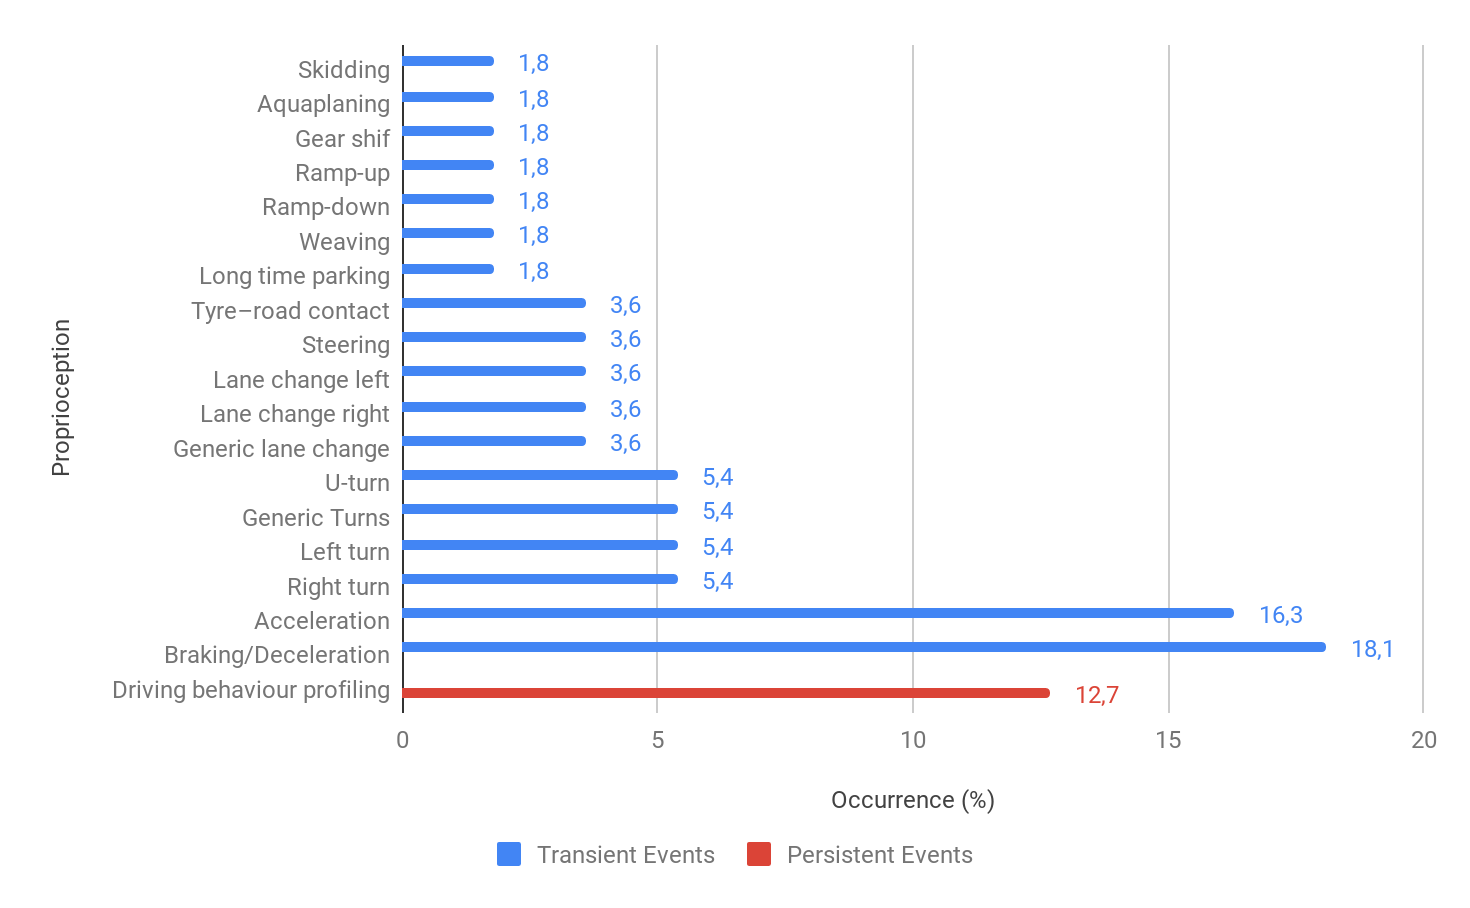
\includegraphics[width=0.95\textwidth]{figuras/fig3_5.png}
   \fonte{O autor.}
\end{figure}

















